\documentclass[12pt, a4paper]{article}

\usepackage[utf8]{inputenc}
\usepackage[T1]{fontenc}
\usepackage[spanish]{babel}
\usepackage{geometry}
\usepackage{graphicx}
\usepackage{hyperref}
\usepackage{listings}
\usepackage{xcolor}
\usepackage{float}
\usepackage{caption}
\usepackage{subcaption}
\usepackage{amsmath}
\usepackage{booktabs}
\usepackage{array}
\usepackage{parskip}
\usepackage{fancyhdr}

\geometry{a4paper, top=3cm, bottom=2.5cm, left=3cm, right=2.5cm}
\graphicspath{{../media/}}

\hypersetup{
    colorlinks=true,
    linkcolor=blue!60!black,
    urlcolor=blue!60!black,
    citecolor=green!50!black,
    pdftitle={Simulación de Coche Autónomo: Percepción},
    pdfauthor={Grupo XI -- MIERA},
}

\definecolor{codegreen}{rgb}{0,0.6,0}
\definecolor{codegray}{rgb}{0.5,0.5,0.5}
\definecolor{codepurple}{rgb}{0.58,0,0.82}
\definecolor{backcolour}{rgb}{0.97,0.97,0.97}
\lstdefinestyle{mystyle}{
    backgroundcolor=\color{backcolour},
    commentstyle=\color{codegreen}, keywordstyle=\color{blue},
    numberstyle=\tiny\color{codegray}, stringstyle=\color{codepurple},
    basicstyle=\ttfamily\footnotesize, breaklines=true,
    keepspaces=true, numbers=left, numbersep=5pt,
    showstringspaces=false, tabsize=2, frame=single,
    rulecolor=\color{gray!30}
}
\lstset{style=mystyle}

\pagestyle{fancy}
\fancyhf{}
\rhead{Percepción en Automática y Robótica -- MIERA 2025/26}
\lhead{Grupo XI}
\cfoot{\thepage}

% ─────────────────────────────────────────────────────────────────────────────
\begin{document}
% ─────────────────────────────────────────────────────────────────────────────

\begin{titlepage}
    \centering
    \vspace*{2cm}
    {\large Universidad de Sevilla \par}
    {\large Máster en Ingeniería de Electrónica, Robótica y Automática (MIERA) \par}
    \vspace{1cm}
    {\large Percepción en Automática y Robótica \par}
    \vspace{2cm}
    \hrule\vspace{0.5cm}
    {\Huge\bfseries Simulación de Coche Autónomo:\\ Detección de Carriles y Señales \par}
    \vspace{0.5cm}\hrule
    \vspace{2cm}
    {\large\itshape Grupo XI \par}
    \vspace{1cm}
    \begin{tabular}{l}
        Samuel Boleslaw Locoche \\[4pt]
        Víctor Javier Granero Gil \\[4pt]
        José Francisco López Ruiz
    \end{tabular}
    \vfill
    {\large Curso 2025--2026 \par}
\end{titlepage}

\tableofcontents
\newpage

\begin{abstract}
Este trabajo presenta el diseño e implementación de un sistema de percepción para un vehículo autónomo simulado en \textbf{CARLA Simulator}, integrado con \textbf{ROS2 Humble} mediante contenedores Docker. El sistema comprende tres módulos principales: detección de líneas de carril mediante una red de segmentación semántica VGG16--U-Net, clasificación de señales de tráfico a través de una CNN entrenada con PyTorch, y un sistema de integración que une ambos módulos con un controlador PID doble para la conducción autónoma. El código fuente, modelos entrenados, datasets y vídeos demostrativos se encuentran en el repositorio público de GitHub: \url{https://github.com/JoseLopez36/Navegacion-Deteccion-Senales}.
\end{abstract}

\newpage

% ═════════════════════════════════════════════════════════════════════════════
\section{Introducción}
% ═════════════════════════════════════════════════════════════════════════════

La conducción autónoma es uno de los retos tecnológicos más ambiciosos de la última década. Para que un vehículo sea capaz de desplazarse sin intervención humana debe ser competente en varias etapas: percepción del entorno, planificación de trayectoria y actuación sobre los sistemas de control. Este trabajo aborda la etapa de \textit{percepción}, responsable de extraer información útil del entorno a partir de los datos sensoriales.

El objetivo del proyecto es desarrollar un sistema de percepción y control básico para un vehículo autónomo simulado en \textbf{CARLA Simulator}, conectado a través de \textbf{ROS2 Humble}. El flujo de funcionamiento diseñado es el siguiente:

\begin{enumerate}
    \item Adquisición de imágenes desde la cámara virtual de CARLA.
    \item Detección de líneas de carril mediante un modelo de segmentación semántica (VGG16--U-Net con TensorFlow/Keras), y estimación del error lateral del vehículo.
    \item Detección y reconocimiento de señales de tráfico mediante una CNN implementada en PyTorch.
    \item Interpretación de las señales para adaptar la velocidad del vehículo.
    \item Publicación de comandos de control hacia CARLA.
\end{enumerate}

Todo el código fuente, modelos entrenados, datasets y material multimedia (imágenes y vídeo demostrativo) están disponibles en el repositorio público de GitHub del proyecto:
\begin{center}
    \url{https://github.com/JoseLopez36/Navegacion-Deteccion-Senales}
\end{center}

\subsection*{Estructura de la memoria}

La memoria se organiza en tres bloques principales:

\begin{description}
    \item[Sección \ref{sec:carriles}: Detección de carriles.]
    Describe el dataset empleado, la arquitectura VGG16--U-Net y los resultados del modelo de segmentación.
    \item[Sección \ref{sec:senales}: Detección y clasificación de señales.]
    Explica el proceso de detección por imagen y el diseño y entrenamiento de la CNN clasificadora.
    \item[Sección \ref{sec:integracion}: Integración en simulación y resultados.]
    Desarrolla la arquitectura software completa en CARLA/ROS2, el control del vehículo y los resultados obtenidos en simulación.
\end{description}

% ═════════════════════════════════════════════════════════════════════════════
\section{Detección de carriles}
\label{sec:carriles}
% ═════════════════════════════════════════════════════════════════════════════

% TODO

% ═════════════════════════════════════════════════════════════════════════════
\section{Detección y clasificación de señales}
\label{sec:senales}
% ═════════════════════════════════════════════════════════════════════════════

% TODO

% ═════════════════════════════════════════════════════════════════════════════
\section{Integración en simulación y resultados}
\label{sec:integracion}
% ═════════════════════════════════════════════════════════════════════════════

Esta sección describe cómo los dos módulos de percepción anteriores se integran dentro de un sistema completo que funciona en simulación. Se presentan el entorno de simulación, la arquitectura software basada en ROS2, los nodos que componen el sistema, el controlador del vehículo y los resultados obtenidos.

% ─────────────────────────────────────────────────────────────────────────────
\subsection{Entorno de simulación: CARLA Simulator}
% ─────────────────────────────────────────────────────────────────────────────

Para el desarrollo y validación del sistema se ha empleado \textit{CARLA Simulator} (\textit{Car Learning to Act}), un simulador de conducción autónoma de código abierto basado en el motor gráfico \textit{Unreal Engine 4}. CARLA proporciona sensores virtuales de gran fidelidad que permiten probar algoritmos de percepción y control sin necesidad de un vehículo real.

El simulador se ejecuta en su versión \textit{0.9.15} dentro de un contenedor Docker con acceso a la GPU de la máquina anfitriona. Las características más relevantes del entorno configurado son:

\begin{itemize}
    \item Mapa: Town04, una autopista con señales de tráfico y carreteras con múltiples carriles.
    \item Vehículo (\textit{ego-vehicle}): modelo basado en Tesla Model 3, controlado desde ROS2.
    \item Sensores disponibles:
    \begin{itemize}
        \item Cámara RGB frontal (\texttt{rgb\_front}): utilizada para detección de carriles y señales.
        \item Cámara de segmentación semántica (\texttt{semantic\_segmentation\_front}): empleada para la generación automática de datasets con \textit{ground truth} perfecto.
        \item Medidor de velocidad (\texttt{speedometer}): velocidad actual del vehículo en m/s.
        \item Cámara exterior (\texttt{rgb\_view}): vista en tercera persona para supervisión visual.
    \end{itemize}
\end{itemize}

La Figura~\ref{fig:vistas_carla} muestra las dos perspectivas principales disponibles en el simulador.

\begin{figure}[H]
    \centering
    \begin{subfigure}[b]{0.48\textwidth}
        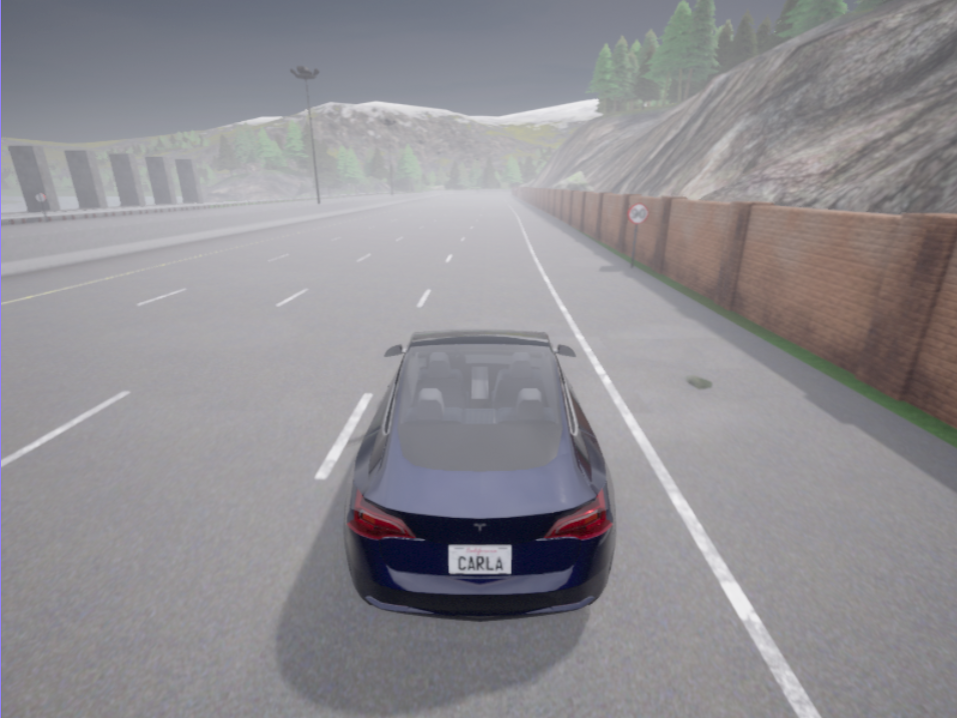
\includegraphics[width=\textwidth]{Vista_Externa.png}
        \caption{Vista exterior (tercera persona).}
    \end{subfigure}
    \hfill
    \begin{subfigure}[b]{0.48\textwidth}
        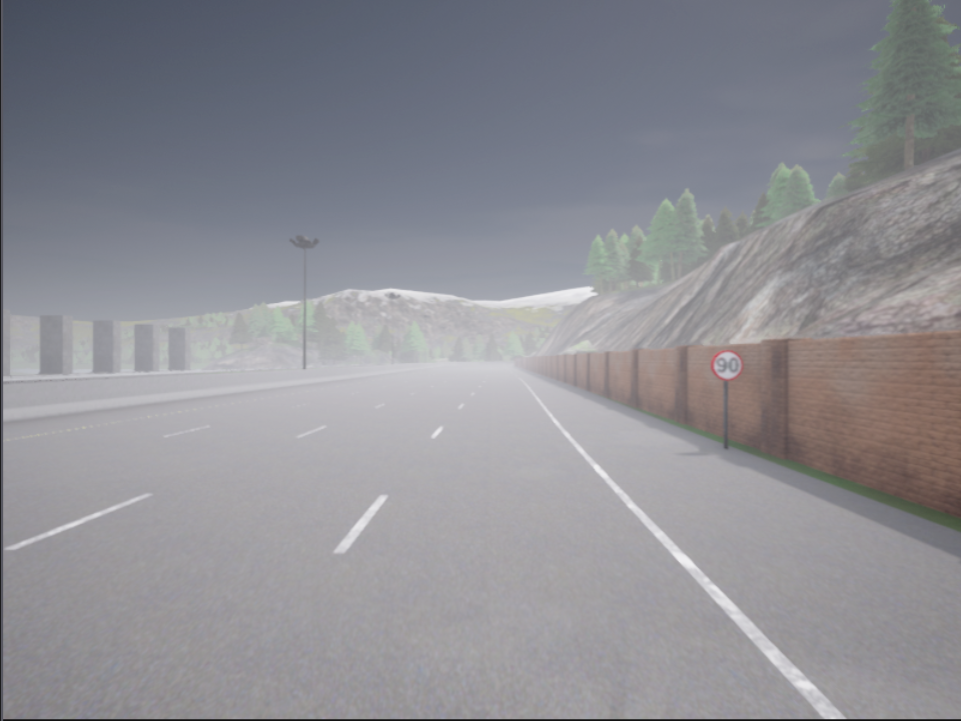
\includegraphics[width=\textwidth]{Vista_Camara_Frontal.png}
        \caption{Cámara frontal del vehículo.}
    \end{subfigure}
    \caption{Perspectivas en CARLA Simulator. Se aprecia el ego-vehicle tipo Tesla y, en la vista frontal, una señal de límite de velocidad a 90~km/h.}
    \label{fig:vistas_carla}
\end{figure}

% ─────────────────────────────────────────────────────────────────────────────
\subsection{Arquitectura del sistema}
% ─────────────────────────────────────────────────────────────────────────────

El sistema completo se articula en tres capas de software que se comunican entre sí a través de una red Docker en modo \textit{host}:

\begin{enumerate}
    \item CARLA Simulator: simulador en contenedor Docker independiente con acceso a la GPU.
    \item CARLA-ROS2 Bridge: puente oficial que traduce los datos de los sensores de CARLA en tópicos ROS2 estándar y convierte los comandos de control ROS2 en actuaciones sobre el vehículo simulado.
    \item Sistema de navegación y percepción: paquete ROS2 propio \\ (\texttt{navegacion\_deteccion\_senales}) que aloja todos los nodos de detección, clasificación y control.
\end{enumerate}

El flujo de información entre los nodos es el siguiente: CARLA publica imágenes en \texttt{/carla/ego\_vehicle/rgb\_front/image} y la velocidad en \\ \texttt{/carla/ego\_vehicle/speedometer}. El \texttt{lane\_detection\_node} procesa esas imágenes y publica el error lateral en \texttt{/lane\_detection/lane\_error}. El \texttt{sign\_detection\_node} publica el límite de velocidad detectado en \texttt{/sign\_detection/speed\_limit}. El \\ \texttt{vehicle\_control\_node} consume ambos tópicos para calcular y publicar los comandos de control en \texttt{/carla/ego\_vehicle/vehicle\_control\_cmd}. Por último, el \\ \texttt{annotation\_generator\_node} agrega toda la información disponible para generar una capa de visualización en tiempo real sobre \textit{Foxglove Studio}.

% ─────────────────────────────────────────────────────────────────────────────
\subsection{Infraestructura: Docker y contenedores}
% ─────────────────────────────────────────────────────────────────────────────

Todo el sistema se orquesta mediante \textbf{Docker Compose}, levantando tres servicios con un único comando desde la raíz del repositorio:

\vspace{0.3cm}
\begin{lstlisting}[language=bash]
xhost +local:docker
docker compose -f tools/docker-compose.yaml up
\end{lstlisting}

La siguiente tabla describe cada uno de los servicios del stack:

\begin{table}[H]
    \centering
    \label{tab:servicios_docker}
    \begin{tabular}{lll}
        \toprule
        \textbf{Servicio} & \textbf{Contenedor} & \textbf{Función} \\
        \midrule
        \texttt{ros\_bridge}  & \texttt{carla\_ros\_bridge}             & Bridge CARLA$\to$ROS2 \\
        \texttt{navegacion}   & \texttt{navegacion\_deteccion\_senales} & Lanzamiento del paquete de ROS2 \\
        \texttt{foxglove}     & \texttt{foxglove\_bridge}               & WebSocket bridge para Foxglove Studio \\
        \bottomrule
    \end{tabular}
\end{table}

La imagen Docker base es \texttt{nvidia/cuda:12.8.0-cudnn-runtime-ubuntu22.04}, sobre la que se instalan:

\begin{itemize}
    \item ROS2 Humble Hawksbill (distribución LTS sobre Ubuntu 22.04).
    \item PyTorch con soporte CUDA~12.8 para inferencia del clasificador de señales en GPU.
    \item ONNX Runtime con soporte GPU, para el modelo de detección de carriles.
    \item Cliente Python de CARLA 0.9.15 y \texttt{carla-ros-bridge} compilado desde el código fuente.
\end{itemize}

El código fuente del paquete ROS2 se monta como volumen dentro del contenedor de navegación, lo que permite que cualquier cambio en el host se aplique de forma inmediata (junto con \texttt{colcon build -{}-symlink-install}) sin necesidad de reconstruir la imagen.

% ─────────────────────────────────────────────────────────────────────────────
\subsection{Nodos ROS2 del sistema}
% ─────────────────────────────────────────────────────────────────────────────

El paquete \texttt{navegacion\_deteccion\_senales} implementa seis nodos ROS2 en Python que se lanzan mediante el fichero \texttt{run.launch.py}.

\subsubsection{Nodo de detección de carriles (\texttt{lane\_detection\_node})}

Este nodo recibe cada \textit{frame} de la cámara frontal, ejecuta la inferencia del modelo VGG16--U-Net exportado en formato ONNX y calcula el error lateral del vehículo respecto al centro del carril, expresado en metros. El error se publica en \\ \texttt{/lane\_detection/lane\_error} (Float32) y el estado completo del carril —incluyendo las coordenadas de las líneas izquierda y derecha— se serializa como JSON en \texttt{/lane\_detection/lane\_state}.

\subsubsection{Nodo de detección de señales (\texttt{sign\_detection\_node})}

El nodo de señales emplea dos entradas: la imagen RGB de la cámara frontal y la imagen de segmentación semántica del mismo punto de vista. La segmentación semántica identifica con precisión los píxeles correspondientes a señales de tráfico (clase de color amarillo en CARLA), obteniendo \textit{bounding boxes} candidatas que se validan por tamaño (\texttt{min\_sign\_area: 150~px}). Sobre el recorte resultante se ejecuta el clasificador CNN, que determina la etiqueta de la señal (\texttt{speed\_limit\_30}, \texttt{speed\_limit\_60}, \texttt{speed\_limit\_90}) y el límite de velocidad en m/s.

\subsubsection{Nodo de control del vehículo (\texttt{vehicle\_control\_node})}

Este nodo cierra el lazo de control: recibe las percepciones de los nodos anteriores y genera los comandos de actuación sobre el vehículo. Opera a 10~Hz e implementa dos controladores PID independientes.

\paragraph{PID de velocidad (control de crucero).}
Regula la velocidad del vehículo en torno a una referencia configurable, inicializada en 2.78~m/s ($\approx$10~km/h). Cuando el nodo de señales detecta un límite de velocidad inferior, la referencia se reduce automáticamente. El error de control es la diferencia entre la velocidad objetivo y la velocidad real medida por el odómetro. La salida del PID se mapea a los canales \textit{throttle} y \textit{brake} normalizados en $[0, 1]$:

\begin{align}
    e_v(t) &= v_{\text{ref}} - v_{\text{actual}} \notag \\
    u_v(t) &= K_{p,v}\,e_v + K_{i,v}\int e_v\,dt + K_{d,v}\,\dot{e}_v \notag \\
    \text{throttle} &= \max(0,\,\min(1,\, u_v)), \quad
    \text{brake} = \max(0,\,\min(1,\,-u_v)) \notag
\end{align}

\paragraph{PID de dirección (mantenimiento de carril).}
Ajusta el ángulo del volante para mantener el vehículo centrado en el carril. La entrada es el error lateral en metros. Para suavizar la respuesta ante el ruido de la máscara de segmentación, se aplica un filtro paso-bajo de primer orden con coeficiente $\alpha = 0.05$ antes de alimentar al PID:

\begin{equation}
    e_{\text{filt}}[k] = \alpha\,e_{\text{raw}}[k] + (1 - \alpha)\,e_{\text{filt}}[k-1]
\end{equation}

La salida del PID, en radianes, se normaliza por el ángulo físico máximo del volante ($\theta_{\max} = 0.6~\text{rad} \approx 34°$) para obtener el valor de dirección normalizado de CARLA en $[-1,1]$. La convención de signo establece que un error positivo (vehículo desplazado a la derecha del carril) genera un giro a la izquierda (dirección negativa).

Ambos PIDs incorporan anti-windup que limita el término integral al rango $[-10, 10]$. Los parámetros finales configurados en \texttt{params.yaml} se recogen en la Tabla~\ref{tab:pid}.

\begin{table}[H]
    \centering
    \caption{Parámetros de los controladores PID (\texttt{params.yaml}).}
    \label{tab:pid}
    \begin{tabular}{lll}
        \toprule
        \textbf{Parámetro} & \textbf{Valor} & \textbf{Descripción} \\
        \midrule
        \texttt{control\_rate}   & 10~Hz          & Frecuencia del bucle de control \\
        \texttt{target\_speed}   & 2.78~m/s       & Velocidad objetivo ($\approx$10~km/h) \\
        \texttt{kp\_throttle}    & 0.30           & Ganancia proporcional de velocidad \\
        \texttt{ki\_throttle}    & 0.05           & Ganancia integral de velocidad \\
        \texttt{kp\_steering}    & 0.20~rad/m     & Ganancia proporcional de dirección \\
        \texttt{ki\_steering}    & 0.02~rad/(m·s) & Ganancia integral de dirección \\
        \texttt{kd\_steering}    & 0.10~rad·s/m   & Ganancia derivativa de dirección \\
        \texttt{max\_steer\_rad} & 0.6~rad        & Ángulo físico máximo del volante \\
        \bottomrule
    \end{tabular}
\end{table}

\subsubsection{Nodo generador de anotaciones (\texttt{annotation\_generator\_node})}

Este nodo actúa como capa de visualización del sistema. En cada \textit{frame} de la cámara frontal, recoge el estado de todos los demás nodos y genera un mensaje \texttt{foxglove\_msgs/\allowbreak ImageAnnotations} que Foxglove Studio superpone sobre la imagen en tiempo real. Las anotaciones incluyen:

\begin{itemize}
    \item Polígono de carril: región semitransparente en verde que cubre el área entre las líneas izquierda y derecha del carril.
    \item Líneas de carril: línea izquierda en amarillo y derecha en cian, con grosor de 6~px.
    \item Vector de desviación: segmento del centro de la imagen al centro del carril estimado; verde si el error es menor de 30~px, rojo si es mayor.
    \item Bounding box de señal: rectángulo con esquinas decorativas y etiqueta de texto; naranja para límites de velocidad, rojo para señales de stop.
    \item HUD de telemetría: textos con el error lateral (m y px), la velocidad actual (km/h) y los valores de \textit{throttle}, \textit{brake} y \textit{steer}.
\end{itemize}

La Figura~\ref{fig:interfaz} muestra la interfaz de Foxglove Studio.

\begin{figure}[H]
    \centering
    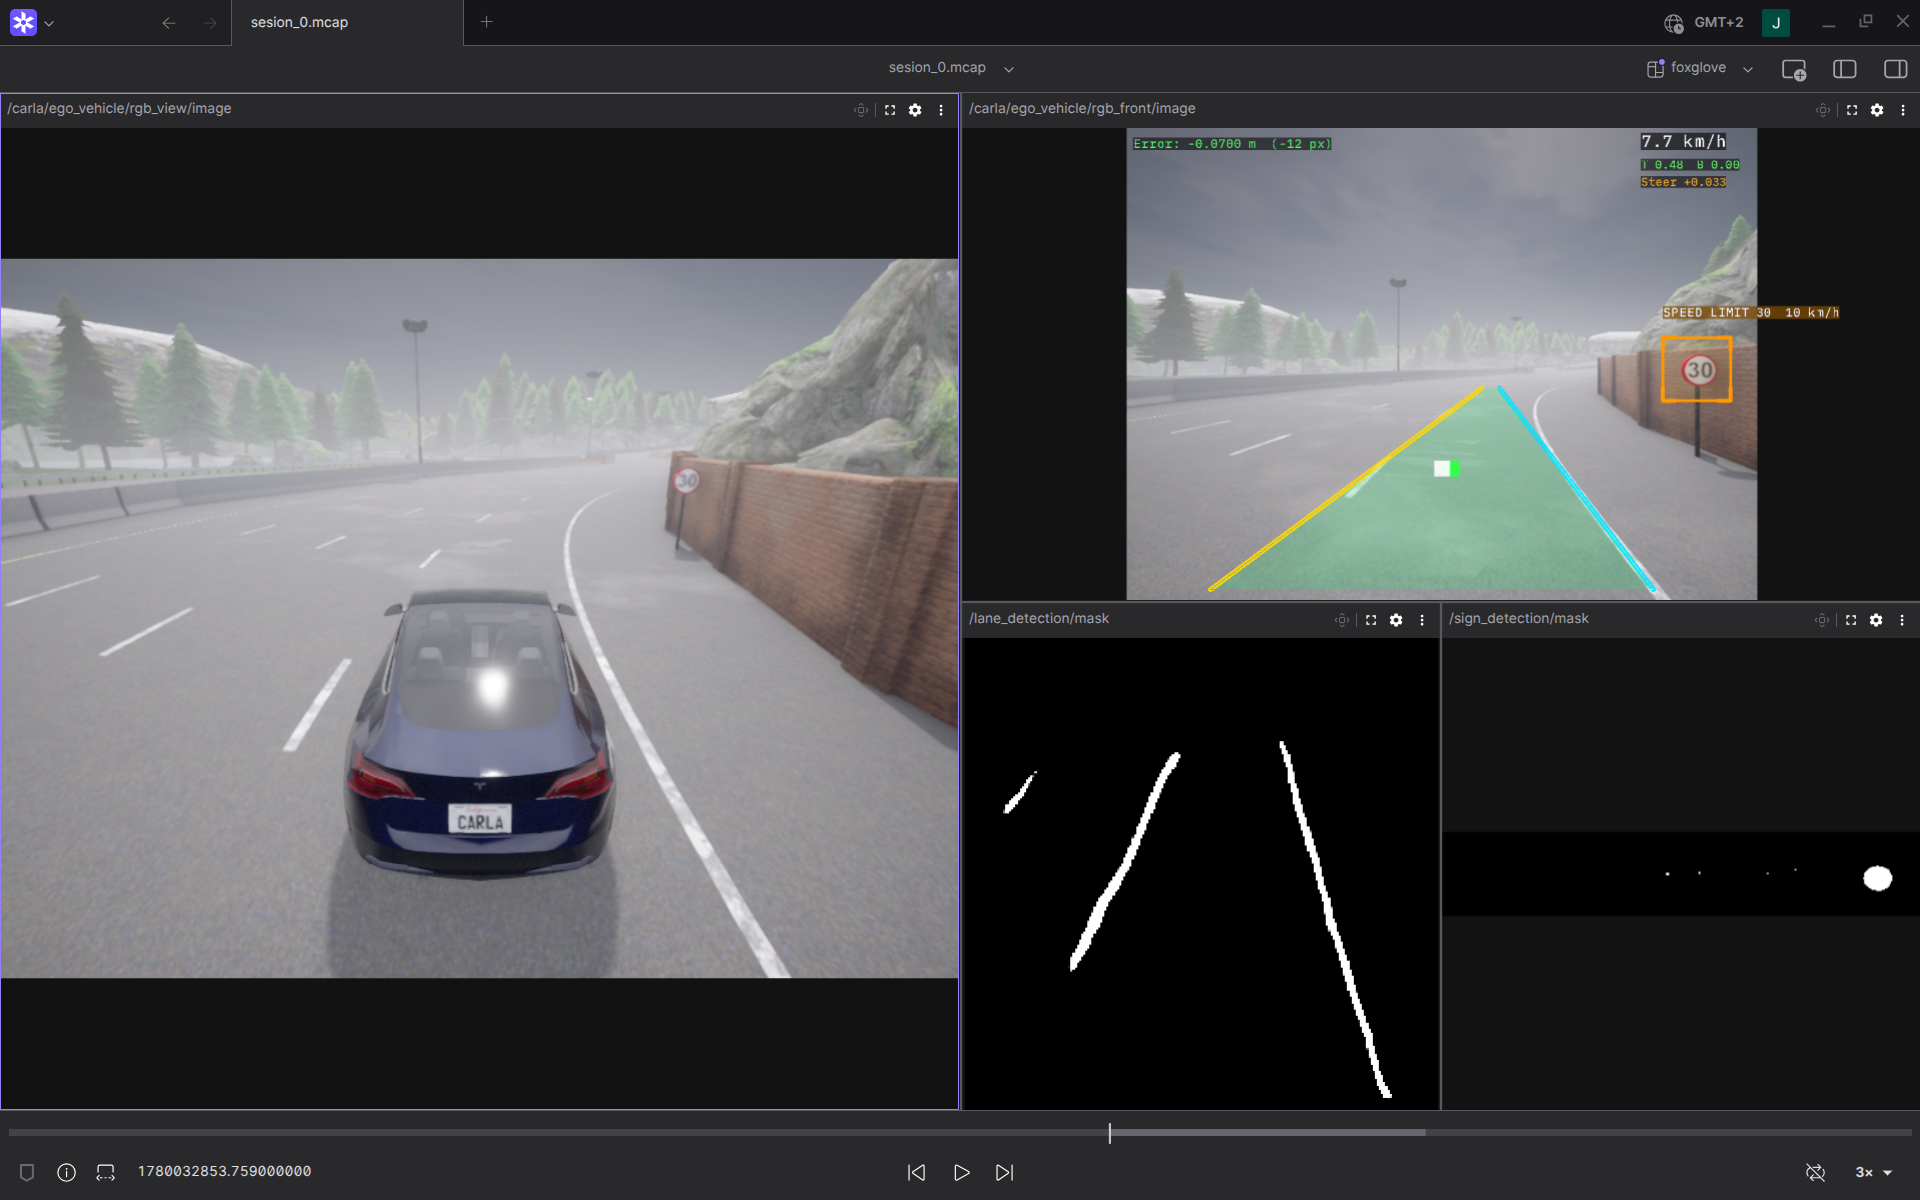
\includegraphics[width=\textwidth]{Interfaz.png}
    \caption{Interfaz de Foxglove Studio durante una sesión de conducción autónoma.}
    \label{fig:interfaz}
\end{figure}

% ─────────────────────────────────────────────────────────────────────────────
\subsection{Generación de datasets sintéticos}
% ─────────────────────────────────────────────────────────────────────────────

Una de las ventajas de trabajar con un simulador como CARLA es la posibilidad de generar datos etiquetados de forma automática. La cámara de segmentación semántica asigna a cada píxel una etiqueta de clase con precisión perfecta, ofreciendo un \textit{ground truth} ideal para entrenar y validar los modelos de percepción sin ningún coste de anotación manual.

El paquete implementa dos nodos de recolección que operan en modo conducción manual (sin \texttt{vehicle\_control\_node}) a una cadencia de 5~Hz:

\paragraph{Dataset de carriles (\texttt{lane\_dataset\_node}).} Detecta las marcas viales en la máscara semántica, las proyecta al espacio RGB y almacena en \texttt{dataset/lanes/} pares de imagen RGB y máscara binaria de \textit{ground truth}.

\paragraph{Dataset de señales (\texttt{sign\_dataset\_node}).} Localiza los píxeles de señales (color amarillo en CARLA), extrae bounding boxes y almacena en \texttt{dataset/signs/} las imágenes RGB junto con ficheros JSON de anotaciones.

Las composiciones Docker para la recolección están en \\ \texttt{tools/docker-compose-lane-dataset.yaml} y \\ \texttt{tools/docker-compose-sign-dataset.yaml}. El repositorio incluye también herramientas de visualización (\texttt{visualize\_lanes\_dataset.py}, \texttt{visualize\_signs\_dataset.py}) y scripts de anotación manual (\texttt{annotate\_signs\_dataset.py}, \texttt{label\_signs\_dataset.py}) para enriquecer el dataset sintético con etiquetas adicionales. Las animaciones del proceso de generación de datos (\texttt{Lanes\_Dataset.gif} y \texttt{Signs\_Dataset.gif}) están disponibles en el repositorio de GitHub.

% ─────────────────────────────────────────────────────────────────────────────
\subsection{Resultados}
% ─────────────────────────────────────────────────────────────────────────────

\subsubsection{Rendimiento en tiempo real}

La siguiente tabla recoge los tiempos de procesamiento medidos durante las sesiones de conducción autónoma en el simulador.

\begin{table}[H]
    \centering
    \label{tab:resultados}
    \begin{tabular}{lll}
        \toprule
        \textbf{Módulo} & \textbf{Latencia media} & \textbf{Frecuencia efectiva} \\
        \midrule
        Detección de carriles  & $\approx$50~ms  & $\approx$20~fps \\
        Detección de señales   & $\approx$13~ms  & $\approx$77~fps \\
        \bottomrule
    \end{tabular}
\end{table}

Ambas latencias se sitúan bien por debajo del período del controlador (100~ms a 10~Hz), lo que garantiza que los comandos de actuación siempre disponen de percepciones actualizadas.

\subsubsection{Entorno de pruebas}

Las pruebas se han realizado sobre el siguiente entorno hardware y software:

\begin{itemize}
    \item CPU: Intel Core i7-13620H.
    \item GPU: NVIDIA GeForce RTX~5070 para portátiles.
    \item Sistema operativo: Ubuntu 22.04 (contenedor Docker).
    \item Framework: ROS2 Humble Hawksbill.
    \item Simulador: CARLA 0.9.15.
\end{itemize}

\subsubsection{Conducción autónoma en simulación}

El sistema completo mantiene el vehículo dentro del carril de forma continuada a velocidades de hasta 30~km/h, adaptando la velocidad cuando detecta señales de límite, pero escaladas a un tercio (i.e. 90~km/h pasa a ser 30~km/h). El vídeo demostrativo del sistema funcionando en tiempo real (\texttt{media/Demo.mp4}) está disponible en el repositorio de GitHub:

\begin{center}
    \url{https://github.com/JoseLopez36/Navegacion-Deteccion-Senales}
\end{center}

% ═════════════════════════════════════════════════════════════════════════════
\section{Conclusiones}
% ═════════════════════════════════════════════════════════════════════════════

Este trabajo ha permitido diseñar e integrar un sistema de percepción completo para la conducción autónoma en simulación, demostrando que la combinación de modelos de \textit{deep learning} con una arquitectura ROS2 modular es una solución eficaz y reproducible. Los resultados obtenidos confirman que el sistema opera en tiempo real con latencias bajas y es capaz de mantener el vehículo dentro del carril mientras respeta los límites de velocidad detectados.

% TODO

\end{document}